\documentclass[11pt,a4paper]{article}
\usepackage[utf8]{inputenc}
\usepackage{amsmath}
\usepackage{amsfonts}
\usepackage{amssymb}
\usepackage{graphicx}
\usepackage{flushend}
\usepackage{indentfirst}
\usepackage{verbatim}
\usepackage{syntax}
\usepackage{geometry}
\geometry{margin=0.5in}
\author{Facundo Molina}

\begin{document}
\title{Proyecto Compiladores: CTds Compiler}
\date{Diciembre, 2015}
\maketitle

\section{Introducción}
\label{sec:intro}
El proyecto consistió en el diseño e implementación de un compilador para el lenguaje CTds, un lenguaje de programación simple muy similar al lenguaje C.  En este documento se presentará la gramática y la semántica del lenguaje CTds, y luego se dará una descripción de cada una de las etapas del desarrollo del compilador, explicando las decisiones de diseño más relevantes.

\section{Gramática del lenguaje CTds}
\label{sec:gramatica}

\begin{grammar}
<program> $\rightarrow$ <class_decl> $^{+}$

<class_decl> $\rightarrow$ \textbf{class} <id> `{' <field_decl>$^{*}$ <method_decl>$^{*}$ `}'

<field_decl> $\rightarrow$ <type> $\lbrace$ <id> $\mid$ <id> `[' <int_literal> `]' $\rbrace ^{+} ,$ `;'

<method_decl> $\rightarrow$ $\lbrace$ <type> $\mid$ \textbf{void} $\rbrace$ <id> `(' \Big[ $ \lbrace$ <type> <id> $\rbrace ^{+} , $ \Big] `)' <body>

<body> $\rightarrow$ <block>
\alt \textbf{extern} `;'

<block> $\rightarrow$ `{'  <field_decl>$^{*}$ <statement>$^{*}$ `}'

<type> $\rightarrow$ \textbf{int} $\mid$ \textbf{float} $\mid$ \textbf{boolean}
 
<statement> $\rightarrow$ <location> <assign_op> <expr> `;'
\alt <method_call> `;'
\alt \textbf{if} `(' <expr> `)' <block> \big[ \textbf{else} <block> \big]
\alt \textbf{for} <id> `=' <expr> `,' <expr> <block> 
\alt \textbf{while} <expr> <block> 
\alt \textbf{return} \big[ <expr> \big] `;'
\alt \textbf{break} `;'
\alt \textbf{continue} `;'
\alt `;'
\alt <block> 

<assign_op> $\rightarrow$ `=' $\mid$ `+=' $\mid$ `-='

<method_call> $\rightarrow$ <id> $\lbrace$ .<id> $\rbrace ^{*}$ `(' \big[ <expr>$^{+},$ \big] `)'

<location> $\rightarrow$ <id> $\lbrace$ .<id> $\rbrace ^{*}$ 
\alt <id> $\lbrace$ .<id> $\rbrace ^{*}$ `[' <expr> `]'

<expr> $\rightarrow$ <location>
\alt <method_call>
\alt <literal>
\alt <expr> <bin_op> <expr>
\alt `-' <expr>
\alt `!' <expr>
\alt `(' <expr> `)'

<bin_op> $\rightarrow$ <arith_op> $\mid$ <rel_op> $\mid$ <eq_op> $\mid$ <cond_op>

<arith_op> $\rightarrow$ `+' $\mid$ `-' $\mid$ `*' $\mid$ `/' $\mid$ `\%'

<rel_op> $\rightarrow$ `<' $\mid$ `>' $\mid$ `<=' $\mid$ `>='

<eq_op> $\rightarrow$ `==' $\mid$ `!='

<cond_op> $\rightarrow$ `&&' $\mid$ `||'

<literal> $\rightarrow$ <int_literal> $\mid$ <float_literal> $\mid$ <bool_literal>

<id> $\rightarrow$ <alpha> <alpha_num>$^{*}$

<alpha_num> $\rightarrow$ <alpha> $\mid$ <digit> $\mid$ `_'

<alpha> $\rightarrow$ `a' $\mid$ `b' $\mid$ ... $\mid$ `z' $\mid$ `A' $\mid$ `B' $\mid$ ... $\mid$ `Z'

<digit> $\rightarrow$ `0' $\mid$ `1' $\mid$ `2' $\mid$ ... $\mid$ `9'

<int_literal> $\rightarrow$ <digit> <digit> $^{*}$

<bool_literal> $\rightarrow$ \textbf{true} $\mid$ \textbf{false}

<float_literal> $\rightarrow$ <digit> <digit> $^{*}$ `.' <digit> <digit> $^{*}$

\end{grammar}

\section{Semántica del lenguaje CTds}
\label{sec:semanticactds}

En esta sección se van a detallar las decisiones de más importancia con respecto a la semántica del lenguaje.

\subsection{General}
\label{subsec:general}

Si bien en la gramática un programa CTds consiste de una lista de declaraciones de clases, y esto es considerado de esa forma en las en las etapas de análisis léxico y sintáctico, a partir de la etapa de análisis semántico se considera que un programa tiene sólo una clase. Esta clase es una lista de declaraciones de atributos seguida de una lista de declaraciones de métodos. Los atributos son variables globales que pueden ser accedidos por cualquier método de la clase. Los métodos representan tanto funcinoes como procedimientos. Además debe haber exactamente un método \textbf{main} sin argumentos, el cuál será el método por donde comenzará la ejecución.

\subsection{Tipos}

Los tipos básicos son \textbf{int}, \textbf{float} y \textbf{boolean}. Se permiten definir arreglos (sólo unidimensionales y de tamaño fijo) para cada uno de los tipos básicos, y son indexados de $0$ a $N-1$, donde $N>0$ es el tamaño. 

Los atributos de una clase pueden de ser de tipos básicos o arreglos, al igual que las variables locales de cualquier bloque.

\subsection{Alcance y visibilidad de los identificadores}
\label{identificadores}

Todos los identificadores deben ser definidos antes de ser utilizados. 

En un punto de un programa CTds existen al menos dos \textit{scopes} válidos, el global (identificadores de atributos y métodos de la clase) y el local a un método (identificadores de variables declaradas en el cuerpo). Dentro de los métodos se pueden introducir \textit{scopes} locales mediante bloques ($\left\langle block \right\rangle$) anidados. Este anidamiento puede causar que un identificador definido en un bloque posterior pueda ocultar alguno definido con el mismo nombre en un bloque previo.

Los nombres de los identificadores son únicos en cada scope. Aunque puede haber atributos o variables con el mismo nombre que un método sin problemas.

\subsection{Locaciones de memoria}
\label{locaciones}

Sólo hay dos clases de locaciones: variables y arreglos (locales y globales). Cada una tiene un tipo. Los arreglos son alocados en el espacio de datos estático del programa (frame de ejecución). 

\subsection{Asignaciones}
\label{asignaciones}

Las asignaciones pueden ser a variables de tipos de básicos o a posiciones de un arreglo. La semántica de las asignaciones define la copia del valor. Una asignación es válida si la locación y la expresión que se intenta asignar tienen el mismo tipo. Las asignaciones de incremento y decremento solo son permitidas para tipos de datos numéricos.

\subsection{Invocación y Retorno de Métodos}
\label{metodos}

La invocación de métodos involucra: pasar el valor de los parámetros actuales a los parámetros formales, ejecutar el cuerpo del método invocado y retornar del método invocado (posiblemente con un resultado).

Los argumentos son pasados por valor. Los parámetros formales son considerados como variables locales del método. 

Tanto los parámetros como el tipo de retorno de un método deben ser de tipo básico. Excepto los métodos que retornan \textbf{void}.

Los métodos que retornan \textbf{void} solamente pueden ser utilizados como una sentencia y además al final deben tener una sentencia \textbf{return} sin una expresión asociada. 

Un método que retorna un resultado puede ser invocado como cualquier expresión. Retornan solo si se alcanza una sentencia \textbf{return} con una expresión del mismo tipo que el tipo de retorno del método.

\subsection{Sentencias de Control}
\label{control}

Las sentencias \textbf{if} y \textbf{while} tienen la semántica estándar. 

En la sentencia \textbf{for} el $\left\langle id \right\rangle$  es la variable índice del ciclo, cuyo valor inicial viene dado por la evualuación de la primera $\left\langle expr \right\rangle$. La segunda $\left\langle expr \right\rangle$ es el valor final de la variable índice, es decir se cicla mientras el valor de $\left\langle id \right\rangle$ sea menor o igual al valor de la segunda $\left\langle expr \right\rangle$. Ambas expresiones deben ser de tipo \textbf{int}. 

Las expresiones siguen las reglas usuales de evaluación. Una locación (variables y elementos de un arreglo) es evaluada al valor que contiene en memoria. Los literales enteros, reales y booleanos evaluan a su valor. En cuanto a los operadores todos tienen el significado usual, teniendo en cuenta de que para los operadores binarios ambos operandos deben ser del mismo tipo, y los operadores relacionales o de igualdad deben devolver un resultado de tipo \textbf{boolean}.

\subsection{Llamadas a funciones externas}
\label{externas}

Se pueden declarar métodos externos reemplazando su cuerpo por la palabra reservada \textbf{extern}.

\subsection{Reglas extras}
\label{extra}

Las siguientes son algunas reglas semánticas adicionales:
\begin{enumerate}
\item Ningún identificador es declarado dos veces en el mismo bloque.
\item Ningún identificador es utilizado antes de ser declarado.
\item Todo programa tiene una única clase, con un único metodo \textbf{main}.
\item Las invocaciones a métodos respetan la aridad con la que los métodos fueron declarados.
\item Las invocaciones a métodos utilizadas como expresión retornan un resultado.
\item La sentencia \textbf{return} solo tiene asociada una expresión si el método retorna un valor, si el método es \textbf{void} no debe tener ninguna.
\item Un $\left\langle id \right\rangle$ usado como una $\left\langle location \right\rangle$ debe estar declarado como parámetro, o como variable local o global.
\item La $\left\langle expr \right\rangle$ en una sentencia \textbf{if} o \textbf{while} debe ser de tipo \textbf{boolean}.
\item Las expresiones iniciales y finales de un \textbf{for} deben ser de tipo \textbf{int}.
\item Las sentencias \textbf{break} y \textbf{continue} solo pueden encontrarse en el cuerpo de un ciclo.
\end{enumerate} 
\section{Etapas} 
\label{sec:etapas}

\subsection{Análisis Léxico} 
\label{subsec:lexico}

El objetivo de esta etapa fue construir el analizador léxico del lenguaje, el cuál a partir del código fuente de un programa CTds debe reconocer que todos los símbolos son correctos, y retornar \textit{tokens}. Comunmente estos \textit{tokens} representan una clase de símbolos del lenguaje, de manera que si, por ejemplo, los símbolos `+',`-',`*',`/' y `\%' forman parte del lenguaje, podemos agruparlos en la clase de símbolos ``Operadores Aritméticos'', y expresarlo en el analizador léxico de la siguiente manera:
\\

\includegraphics[width=18.5cm,height=2.8cm]{lexical1.png} \\ 
 
Donde para cada uno de los operadores aritméticos se retorna el \textit{token} \textbf{ARITHMETHICAL_OP}. Esta codificación se puede repetir análogamente para el resto de clases de símbolos del lenguaje (operadores relacionales, operadores lógicos, palabras reservadas, etc). Como para etapas posteriores es conveniente tener identificados cada uno de los símbolos, es decir, saber si el operador que se está utilizando es exactamente `+', `-' o cualquiera de los otros, se optó por tener \textit{tokens} individuales por cada uno de los símbolos:
\\

\includegraphics[width=17cm,height=2.8cm]{lexical2.png} \\ 

Y del mismo modo, cada símbolo del lenguaje (operadores relacionales, palabras reservadas, etc) tiene asociado un \textit{token} propio.

La herramienta utilizada para generar el analizador léxico fue JFlex, la cuál a partir de una especificación, como la presentada en el código previo, genera el scanner \textit{CTdsScanner} que es capaz de reconocer los símbolos y retornar el \textit{token} correspondiente para cada uno de ellos. Por ejemplo, para una cadena de símbolos que represente una asignación:
\begin{center}
	$x = y+2 ;$
\end{center}
\textit{CTdsScanner} generaría la cadena de \textit{tokens}:
\begin{center}
	$ID \ ASSIGN\_OP \ ID \ PLUS \ INT\_LITERAL \ SEMI\_COLON$
\end{center}

\subsubsection{Testing}

Fueron implementados una serie de tests para el analizador léxico, proporcionando en un archivo secuencias de símbolos válidos para el lenguaje y en otro archivo la secuencia de tokens esperados. Y luego del análisis los tokens retornados debían ser exactamente los mismos que los tokens esperados. Se implementaron tests de acuerdo a la clase de tokens a reconocer, es decir, para \textit{literales}, \textit{operadores}, \textit{keywords}, \textit{delimitadores}, \textit{identificadores}, etc.

\subsection{Análisis Sintáctico} 
\label{subsec:sintactico}
A partir de los \textit{tokens} que se obtienen al finalizar el análisis léxico, se realiza el análisis sintáctico, el cuál consiste en reconocer que las sentencias están construidas correctamente de acuerdo a la especificación del lenguaje, es decir, que los símbolos aparecen en el orden correcto. 

Para reconocer las frases es necesario un parser, y la herramienta utilizada para generarlo fue CUP. A partir de la especificación de la gramática, en una forma muy similar a la presentada en la sección~\ref{sec:gramatica}, CUP genera el parser \textit{CTdsParser} del lenguaje. La salida de este parser es el árbol de parsing, donde cada uno de los nodos se corresponde con algún símbolo de la gramática.
\\

\includegraphics[width=18cm,height=6.5cm]{sintactic1.png} \\ 

En la figura se observa la parte de la definición de la gramática correspondiende a ``statements''. Si bien las tres primeras sentencias, correspondientes a asignaciones, podrían haber sido expresadas en sólo una con un operador genérico, ya que lo único que cambia entre ellas el operador de asignación, se realizó de esta manera para obtener mayor precisión a la hora de constuir el árbol de parsing. A modo de ejemplo, para la cadena de tokens del ejemplo de la sección \ref{subsec:lexico}:
\begin{center}
	$ID \ ASSIGN\_OP \ ID \ PLUS \ INT\_LITERAL \ SEMI\_COLON$
\end{center}
que se corresponde con la primer regla de ``statements'':	
\begin{center}
\includegraphics[width=9cm,height=0.6cm]{sintactic2.png} \\
\end{center}
en el árbol de parsing tendríamos:
\\
\begin{center}
\includegraphics[width=13cm,height=6.5cm]{ctdsparsing.png} \\
\end{center}

De haber tenido la tres primeras reglas generalizadas en sólo una, se debería haber hecho algún procesamiento extra para determinar de qué operador se trataba. En esta etapa la mayoría de las decisiones tuvieron que ver con esa misma idea, tratar de tener la mayor información posible a la hora de constuir el árbol.

Para la construcción del AST se diseñó la siguiente jerarquía de clases:
\\
\begin{flushleft}
	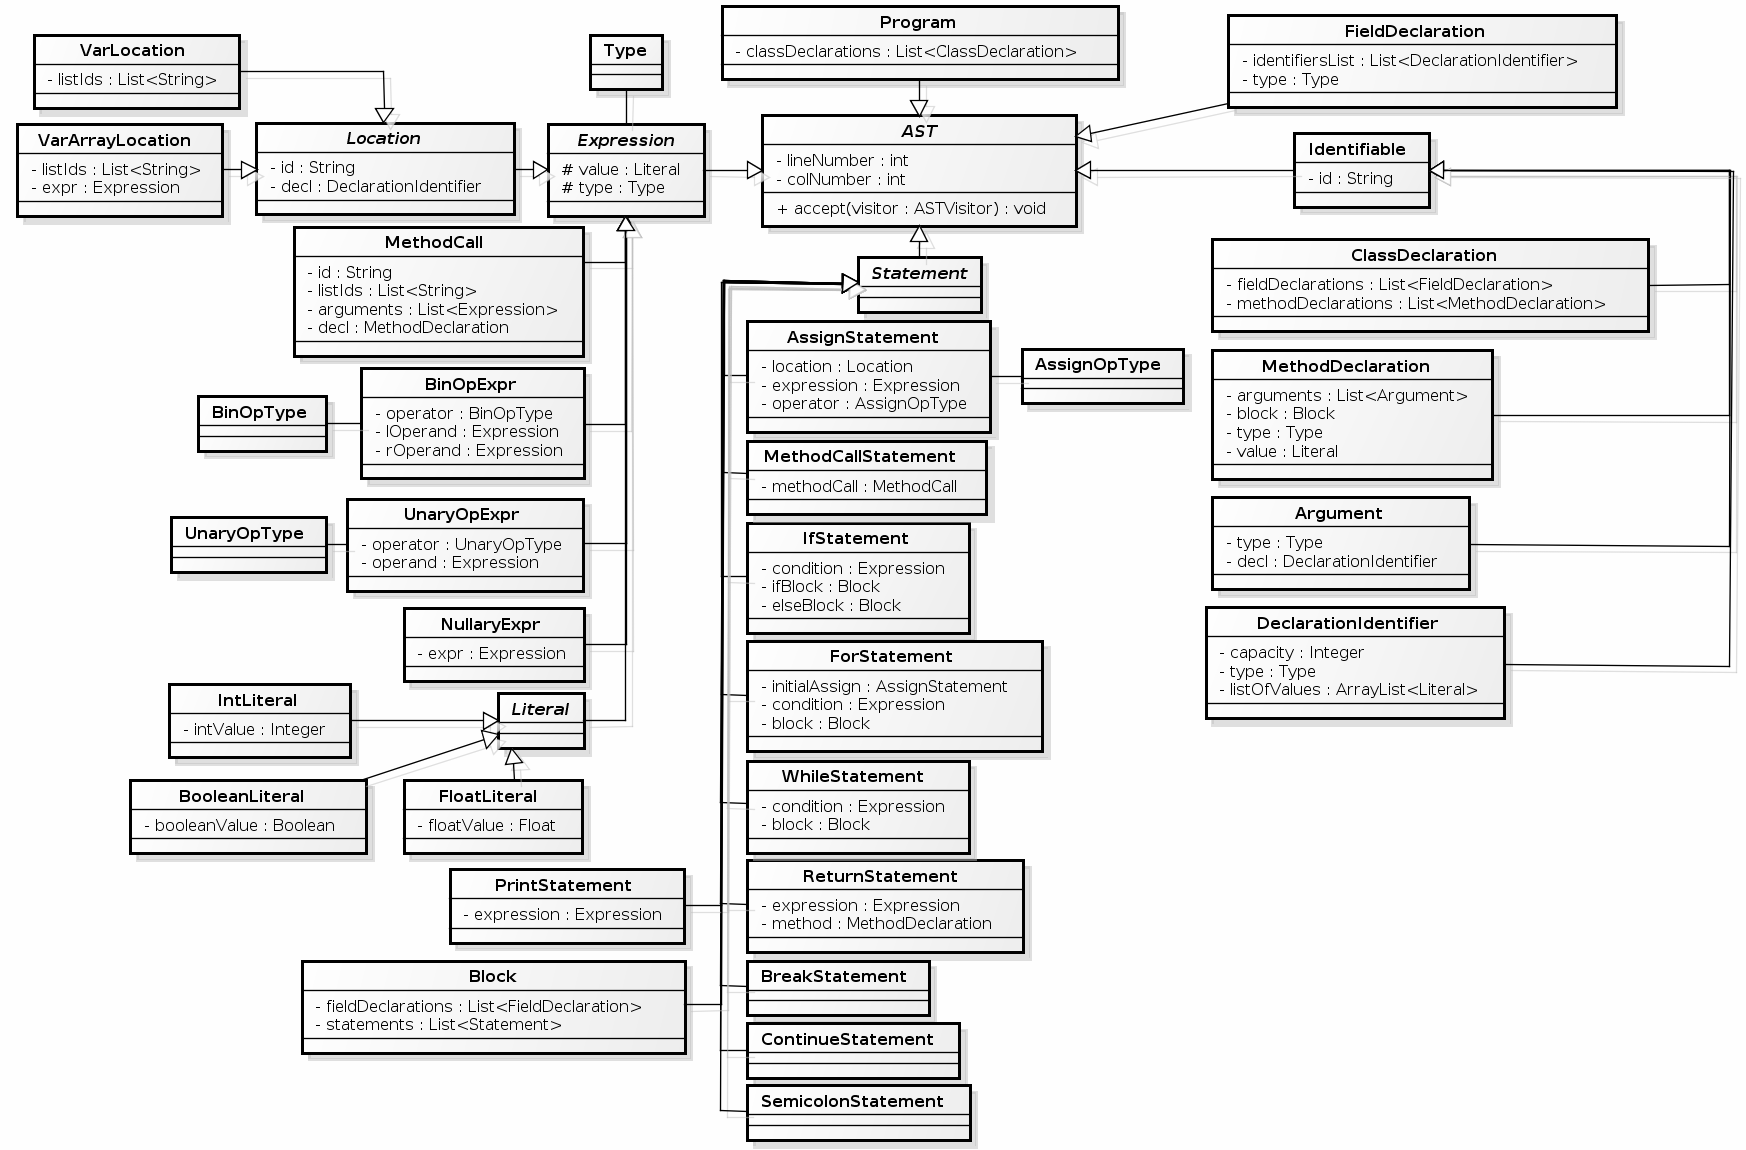
\includegraphics[width=19.6cm,height=18cm]{ASTDiagram.png}
\end{flushleft}

Basicamente cuando se genera el AST, la raíz es un elemento \textit{Program}, a partir del cuál se puede comenzar a acceder a objetos \textit{ClassDeclaration}, luego a \textit{FieldDeclaration} y \textit{MethodDeclaration}, a partir de estos últimos a elementos \textit{Argument} y al objeto \textit{Block}, y luego a elementos \textit{Statement}, así sucesivamente a cada nodo.

\subsubsection{Testing}

Los tests implementados para comprobar el correcto funcionamiento del parser, fueron realizados a partir de archivos con cadenas de texto, algunas pertenecientes al lenguaje CTds y otras no pertenecientes al lenguaje (con errores sintácticos), y verificando que para las pertenecientes al lenguaje el parser la reconoce correctamente, y para aquellas no pertenecientes se obtienen errores. 

\subsection{Análisis Semántico} 
\label{subsec:semantico}

Esta etapa consiste en chequear las reglas semánticas del lenguaje, entre las que se encuentran la compatibilidad de tipos, la correcta declaración y uso de los identificadores, y todas las detalladas en la sección ref{sec:semanticactds}. Para verificar estas reglas se implementaron \textit{visitors} del AST generado durante el parsing: 

\subsubsection{Mains}
\label{mains}
El visitor \textit{CheckMainVisitor} es el más simple de todos, ya que su objetivo es determinar la cantidad de métodos \textbf{main} para comprobar si hay exactamente un método \textbf{main} (es lo esperado) o más de uno. Para implementarlo, sólo es necesario mirar cada nodo del árbol que se corresponda con la declaración de un método y determinar si su identificador es \textbf{main} o no.
 
\subsubsection{Declaraciones}
\label{subsec:decls}

El visitor \textit{CheckDeclarationVisitor} permite determinar si los identificadores son duplicados o no, si han sido correctamente declarados antes de ser utilizados, etc. La idea es utilizar una tabla de símbolos a modo de pila, donde a medida que se va profundizando un nuevo nivel en el AST (pasamos de  un nodo que representa una $\left\langle class\_decl \right\rangle$ a otro que representa una $\left\langle field\_decl \right\rangle$, o de uno que representa una $\left\langle method\_decl \right\rangle$ a otro que representa un $\left\langle statement \right\rangle$) de asignación, etc) se va apilando el segundo nodo en la pila. El nivel actual, por ejemplo el de $\left\langle class\_decl \right\rangle$, es visto como una lista, donde se van agregando los nodos que no representan un nuevo nivel con respecto al actual, es decir nodos que representan $\left\langle class\_decl \right\rangle$. 

De esta manera, para detectar duplicados simplemente es necesario recorrer la lista del nivel actual y comprobar que no existe ningún identificador igual que el identificador del elemento actual. Y para verificar si un identificador ha sido declarado correctamente antes de ser utilizado hay que buscarlo en los niveles anteriores de la pila. 

\paragraph{Testing.} Para el testing del \textit{CheckDeclarationVisitor} se implementaron tests con programas CTds correctos, para los cuáles el \textit{visitor} no debe encontrar errores, y tests con programas CTds con errores semánticos sobre declaraciones, es decir, con identificadores duplicados, variables no declaradas, métodos sin sentencia \textbf{return}, etc.


\subsubsection{Tipos}
\label{subsec:tipos}

El visitor \textit{CheckTypeVisitor} determina si los tipos han sido definidos correctamente de acuerdo a la semántica: 
\begin{itemize}
	\item si las asignaciones a locaciones respetan el tipo que fue utilizado en la declaración de las locaciones
	\item si las operaciones son realizadas entre expresiones de tipos equivalentes
	\item si los operadores en las expresiones son compatibles con los tipos
	\item si los métodos retornan expresiones del mismo tipo que el de su declaración
	\item si los parámetros actuales tienen el mismo tipo que los parámetros formales
	\item si las expresiones de las sentencias condicionales tienen tipo \textbf{boolean}
\end{itemize}

De la misma manera que para las declaraciones, se usa una tabla de símbolos a modo de pila. Para la visita de cada nodo del AST la forma de proceder es la siguiente: se realiza el chequeo de tipos si es necesario, por ejemplo en la condición de un \textbf{if} (el tipo debe ser \textbf{boolean}), y si no hay errores se continúa visitando el interior del nodo ($\left\langle block \right\rangle$ en el caso del \textbf{if}). Si se encuentra algún error, directamente se agrega a la lista de errores de tipo y no se visita el interior del nodo actual. Para los casos en los que no es necesario un chequeo de tipos, por ejemplo una  $\left\langle field\_decl \right\rangle$, se agrega el nodo a la pila (en el caso de declaraciones, ya que sus identificadores pueden ser necesarios), y se visita el nodo siguiente.

\paragraph{Testing.} Para el testing del \textit{CheckTypeVisitor} se implementaron tests con programas CTds correctos y tests con programas CTds con errores de tipos, y verificando que en este último caso los errores introducidos son detectados.

\subsection{Intérprete} 
\label{subsec:interprete}

En esta etapa se diseñó e implementó un intérprete de CTds, \textit{InterpreterVisitor}, el cuál a partir del AST generado en el parsing, y luego de comprobar que el programa no tiene errores semánticos (es decir, ejecutando los visitors \textit{CheckMainVisitor}, \textit{CheckDeclarationVisitor} y \textit{CheckTypeVisitor}), comienza desde el método \textbf{main} a ejecutar cada una de las sentencias respetando la semántica de cada una:
\begin{itemize}
\item para las asignaciones, se evalua la expresión y se asgina el valor en la locación.
\item para las expresiones unarias, se evalua la expresión y luego se evalua el resultado con el operador
\item para las expresiones binarias, se evalua ambas expresiones y luego se aplica el operador sobre el valor de cada una de ellas
\item para las llamadas a métodos se evaluan los argumentos, se asignan los valores a los parámetros formales y se comienza a ejecutar las sentencias del cuerpo del método invocado
\item para las sentencias \textbf{if} se evalua la expresión booleana, si el resultado es \textbf{true} se ejecutan las sentencias del bloque del \textbf{if}, si es \textbf{false} se ejecutan las sentencias del bloque del \textbf{else}.
\item para las sentencias \textbf{while} mientras la evaluación de la expresión sea \textbf{true} se ejecutan las sentencias del cuerpo del ciclo.
\end{itemize}
Se omiten algunas sentencias ya que su ejecución es similar a alguna de las descriptas. 

\subsection{Generación de Código Intermedio} 
\label{subsec:genci}

En la generación de código intermedio se implementó el \textit{IntermediateCodeGeneratorVisitor} con el objetivo de generar una representación intermedia de bajo nivel del código CTds, a partir de la cuál será posible generar el código objeto del programa. 

Para esta etapa se diseñó una jerarquía de clases para representar las sentencias del código intermedio:
\\

\includegraphics[width=16cm,height=10cm]{icgdiagram.png}

La idea es, a partir del AST del programa, generar una lista de  \textit{IntermediateCodeStatement}, donde cada elemento de la lista puede ser:
\begin{itemize}
\item \textit{IntermediateCodeStatement}: por ejemplo para la instrucción \textit{RET}, que en ocasiones no requiere expresiones.
\item \textit{OneAddressStatement}: para las instrucciones \textit{JUMPF} (Salto por falso) y \textit{JUMP} (Salto incondicional) que solo requieren un label al cuál saltar. O la instrucción \textit{PUSH} que necesita la expresión que se desea agregar a la pila. 
\item \textit{TwoAddressStatement}: para la instrucción \textit{ASSIGN} que necesita dos expresiones, una conteniendo la locación y la otra conteniendo la expresión que se va a asignar. O también la instrucción \textit{CALL}, que requiere la expresión de la llamada al método y la locación en donde almacenar el resultado.
\item \textit{ThreeAdressStatement}: para las instrucciones \textit{ADDI} (suma de enteros) y \textit{ADDF} (suma de flotantes), que utilizan dos las dos expresiones a sumar y además la locación en donde se va a retornar el resultado.
\end{itemize}

Todas las instrucciones mencionadas corresponden a objetos del tipo \textit{IntermediateCodeInstruction}.

También se utilizaron dos pilas, una para ir apilando los labels de inicio de los nodos y otra para los labels de fin. Esto es útil para algunos nodos, por ejemplo los que representan \textbf{for} o \textbf{while}, ya que para algunas sentencias, como \textbf{break} o \textbf{continue}, es necesario saber el label de inicio o fin. 

\subsection{Generación de Código Objeto} 
\label{subsec:genco}

Para generar el código assembler a partir del código intermedio se implementó \textit{AssemblerCodeGenerator}. El cuál lo que hace es ir recorriendo cada elemento  de la lista de \textit{IntermediateCodeStatement} creada en la etapa anterior y generando las instrucciones assembler necesarias para representar cada \textit{IntermediateCodeInstruction}. A continuación se muestran algunos ejemplos del código assembler generado para distintas sentencias:
\subsubsection{Asignaciones}
\begin{itemize}
	\item CTds:
		\begin{flushleft}
			$\ \ \ \ x = 2 ;$
		\end{flushleft}
	\item Código intermedio:
		\begin{flushleft}
			$\ \ \ \ ASSIGN \ \ 2 \ \ x$
		\end{flushleft}
	\item Assembler:
		\begin{flushleft}
			$\ \ \ \ movl \ \ \$2, \ \ \%ebx $ \\
			$\ \ \ \ movl \ \ \%ebx, \ \ -4(\%ebp)$	
		\end{flushleft}
		Donde $-4(\%ebp)$ es la dirección de memoria reservada para $x$.
\end{itemize}
\subsubsection{Operación aritmética con enteros}
\label{subsec:enteros}
\begin{itemize}
	\item CTds:
		\begin{flushleft}
			$\ \ \ \ y = x + 2 ;$
		\end{flushleft}
	\item Código intermedio:
		\begin{flushleft}
			$\ \ \ \ ADDI \ \ x \ \ 2 \ \ t0$ \\
			$\ \ \ \ ASSIGN \ \ t0 \ \ y$
		\end{flushleft}
		Donde $t0$ es una variable temporal.
	\item Assembler:
		\begin{flushleft}
			$\ \ \ \ movl \ \ -4(\%ebp), \ \ \%ebx $ \\
			$\ \ \ \ addl \ \ \$2, \ \ \%ebx$ \\
			$\ \ \ \ movl \ \ \%ebx, \ \ -12(\%ebp)$ \\
			$\ \ \ \ movl \ \ -12(\%ebp), \ \ \%ebx$ \\
			$\ \ \ \ movl \ \ \%ebx, \ \ -8(\%ebp)$	
		\end{flushleft}
		Donde $-4(\%ebp)$, $-8(\%ebp)$ y $-12(\%ebp)$ son las direcciones de memoria de $x$, $y$ y $t0$ respectivamente. Notar que para el resto de las operaciones aritméticas sólo cambia la instrucción $addl$ por la correspondiente.
\end{itemize}
\subsubsection{Operación aritmética con flotantes}
\begin{itemize}
	\item CTds:
		\begin{flushleft}
			$\ \ \ \ y = x + 2.0 ;$
		\end{flushleft}
	\item Código intermedio:
		\begin{flushleft}
			$\ \ \ \ ADDF \ \ x \ \ 2.0 \ \ t0$ \\
			$\ \ \ \ ASSIGN \ \ t0 \ \ y$
		\end{flushleft}
		Donde $t0$ es una variable temporal.
	\item Assembler:
		\begin{flushleft}
			$\ \ \ \ flds \ \ -4(\%ebp) $ \\
			$\ \ \ \ fadds \ \ .label2$ \\
			$\ \ \ \ fstps -12(\%ebp)$ \\
			$\ \ \ \ movl \ \ -12(\%ebp), \ \ \%ebx$ \\
			$\ \ \ \ movl \ \ \%ebx, \ \ -8(\%ebp)$	
		\end{flushleft}
		Donde $-4(\%ebp)$, $-8(\%ebp)$ y $-12(\%ebp)$ son las direcciones de memoria de $x$, $y$ y $t0$ respectivamente, y $.label2$ es el label para la constante $2.0$. Notar que para el resto de las operaciones aritméticas sólo cambia la instrucción $fadds$ por la correspondiente.
\end{itemize}
\subsubsection{Declaraciones de métodos}
\begin{itemize}
	\item CTds:
		\begin{flushleft}
			$\ \ \ \ \textbf{int} \ sum(\textbf{int} \ a,\textbf{int} \ b) \{$ \\
			$\ \ \ \ \ \ \ \ \textbf{return} \ a + 	b \ ;$ \\
			$\ \ \ \ \}$
		\end{flushleft}
	\item Código intermedio:
		\begin{flushleft}
			$\ \ \ \ INITML \ \ sum$ \\
			$\ \ \ \ RESERVE \ \ amount$ \\
			$\ \ \ \ ADDI \ \ a \ \ b \ \ t0$ \\
			$\ \ \ \ RET \ \ t0$
		\end{flushleft}
		$INITML$ es la instrucción que representa el inicio de la declaración de un método, cuyo nombre en este caso es $sum$ y $RESERVE$ es la instrucción utilizada para reservar enla pila tanto espacio como el valor de $amount$.
	\item Assembler:
		\begin{flushleft}
			$\ \ \ \ .globl \ \ sum$ \\
			$\ \ \ \ .type \ \ sum, \ \ @function $ \\
			$sum:$ \\
			$\ \ \ \ pushl \ \ \%ebp$ \\
			$\ \ \ \ movl \ \ \%esp, \ \ \%ebp$ \\
			$\ \ \ \ movl \ \ 8(\%ebp), \ \ \%ebx$ \\
			$\ \ \ \ addl \ \ 12(\%ebp), \ \ \%ebx$ \\
			$\ \ \ \ movl \ \ \%ebx, \ \ -4(\%ebp)$ \\
			$\ \ \ \ movl \ \ -4(\%ebp), \ \ \%eax$ \\
			$\ \ \ \ leave$ \\
			$\ \ \ \ ret$	
		\end{flushleft}
		Donde $8(\%ebp)$ y $12(\%ebp)$ son las direcciones de memoria de los parámetros $a$ y $b$ respectivamente, y $-4(\%ebp)$ es la dirección de memoria $t0$. Los resultados de los métodos siempre son almacenados en el registro $eax$. 
\end{itemize}
\subsubsection{Invocaciones a métodos}
\begin{itemize}
	\item CTds:
		\begin{flushleft}
			$\ \ \ \ x = sum(x,y);$
		\end{flushleft}
	\item Código intermedio:
		\begin{flushleft}
			$\ \ \ \ PUSH \ \ y$ \\
			$\ \ \ \ PUSH \ \ x$ \\			
			$\ \ \ \ CALL \ \ sum \ \ t1$ \\
			$\ \ \ \ ASSIGN \ \ t1 \ \ x$
		\end{flushleft}
		Donde $t1$ es una variable temporal.
	\item Assembler:
		\begin{flushleft}
			$\ \ \ \ pushl \ \ -8(\%ebp)$ \\
			$\ \ \ \ pushl \ \ -4(\%ebp)$ \\
			$\ \ \ \ call \ \ sum$ \\
			$\ \ \ \ movl \ \ \%eax, \ \ -12(\%ebp)$ \\
			$\ \ \ \ movl \ \ -12(\%ebp), \ \ \%ebx$ \\ 
			$\ \ \ \ movl \ \ \%ebx, \ \ -4(\%ebp)$	
		\end{flushleft}
		Donde $-4(\%ebp)$  $-8(\%ebp)$ y $-12(\%ebp)$ son las direcciones de memoria de $x$, $y$ y $t0$ respectivamente. Mediante $call \ sum$ se comienzan a ejecutar las instrucciones del cuerpo del método $sum$ descriptas anteriormente.
\end{itemize}

\paragraph{Compilación.} Ya que el código generado por el  \textit{AssemblerCodeGenerator} es el mismo que el generado por el lenguaje C, el \textit{GNU Assembler}, puede ser compilado utilizando \textit{gcc}. De esta manera también se puede linkear fácilmente código escrito en otros lenguajes.

\subsection{Análisis y Optimización} 
\label{subsec:opt}

El objetivo de esta etapa es analizar el código para aplicar distintas posibles optimizaciones tratando de reducir los tiempos de ejecución. Algunas de las posibles optimizaciones son:
\begin{itemize}
	\item Resolver operaciones entre expresiones constantes. Una vez realizados los chequeos semánticos necesarios, aquellas operaciones que involucren solo constantes se pueden calcular y sólo dejar el valor total de la expresión. De esta manera se pueden reducir la cantidad de cálculos en etapas posteriores.
	\item Reducir la cantidad de instrucciones $movl$ generadas. En muchas ocaciones, al utilizar variables temporales como en el ejemplo \textbf{Operación aritmética con enteros} de la sección anterior, se generan instrucciones $movl$ innecesarias. 
	\item No generar código de bajo nivel para sentencias que no se ejecutan a través de ninguna traza. Por ejemplo, en una sentencia \textbf{if} con una condición que siempre evalua a \textbf{true}, las sentencias del cuerpo del \textbf{else} nunca se ejecutarán, por lo tanto no es necesario generar código para esas sentencias.
\end{itemize}

Si bien esta etapa no se llevó a cabo, es necesario notar hay que ser precisos en el análisis y las optimizaciones que se deseen efectuar, ya que realizar un excesivo análisis del código puede llevar a elevar los tiempos de compilación, y también no ser precisos en la optimización, más aún cuando se trata de código de bajo nivel, puede llevar a generar programas que dejen de respetar la semántica del lenguaje. 

\section{Resultado final} 
\label{sec:concl}

Después de llevar a cabo cada una de las etapas del desarrollo del compilador $CTdsCompiler$, se concluyó con la siguiente estructura:
\begin{center}
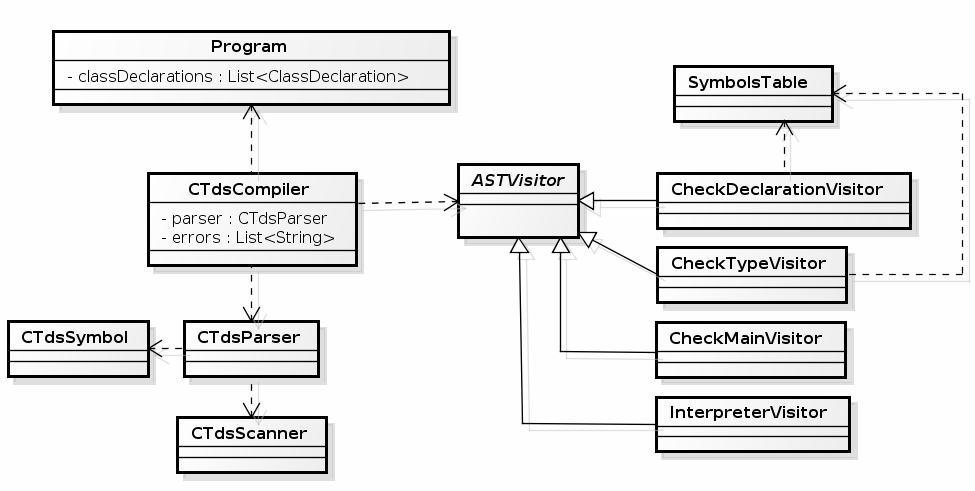
\includegraphics[width=14cm,height=8cm]{CTdsCompilerDiagram.png}
\end{center}
donde el orden de ejecución del compilador es básicamente el mismo de las etapas, es decir:
\begin{enumerate}
	\item Análisis Léxico: \textit{CTdsScanner}
	\item Análisis Sintáctico: \textit{CTdsParser}
	\item Análisis Semántico: \textit{CheckDeclarationVisitor}, \textit{CheckTypeVisitor} y \textit{CheckMainVisitor}
	\item Generación de Código Intermedio: \textit{IntermediateCodeGeneratorVisitor}
	\item Generación de Código Objeto: \textit{AssemblerCodeGenerator}
\end{enumerate}
y sólo se va continuando a la etapa siguiente si no se obtuvo ningún error en la etapa anterior.
\end{document}